\chapter{Literature Review}
\label{ch:literature}

This chapter reviews the works on which the design of this project is directly based.

\section{Reinforcement Learning and Policy Optimisation}
In reinforcement learning an agent interacts with an environment, observes states, selects actions and
receives rewards; the objective is a policy that maximises the expected discounted return. For continuous
control, policy-gradient methods optimise a parameterised stochastic policy directly. Proximal Policy
Optimisation (PPO) \cite{schulman2017proximal} restricts each policy update with a clipped probability ratio,
so that the new policy cannot move too far from the policy that collected the data. This makes learning stable
while allowing several optimisation epochs on the same batch of experience. The quality of a policy-gradient
update depends strongly on the estimate of the advantage, i.e.\ how much better an action was than expected.
Generalised Advantage Estimation (GAE) \cite{schulman2016gae} computes this estimate as an exponentially
weighted sum of temporal-difference errors, with a parameter $\lambda$ that trades bias against variance. PPO
with GAE is the optimisation method used in this project.

\section{Multi-Agent Reinforcement Learning for Cooperative Tasks}
When several agents learn together, the environment becomes non-stationary from the point of view of each agent.
Yu et al.\ \cite{yu2022surprising} showed that PPO, often regarded as a single-agent method, is a strong
algorithm for cooperative multi-agent problems when it is combined with parameter sharing among homogeneous
agents and with a small number of implementation choices such as few epochs per batch, a clip parameter of at
most 0.2 and large batches. They compare a local value function (independent PPO) with a centralised value
function (MAPPO) that uses global information during training only. Following this study, our policy is shared
by all drones and trained with PPO and a local critic; the centralised critic is left as an option for future
comparison.

\section{Deep Reinforcement Learning for Quadrotor Swarms}
Batra et al.\ \cite{batra2021decentralized} trained a decentralised policy for quadrotor swarms end-to-end with
PPO (Figure~\ref{fig:lit_batra}). Each drone encodes its own state with a self encoder and the relative positions
and velocities of its neighbours with a permutation-invariant neighbour encoder (deep sets or attention), and the
same policy is shared by all drones. The trained swarms keep and change formations, and in one experiment
re-establish their formation around moving spherical obstacles. The paper also separates collision and formation
measurements, which our evaluation adopts.

\begin{figure}[htbp]
  \centering
  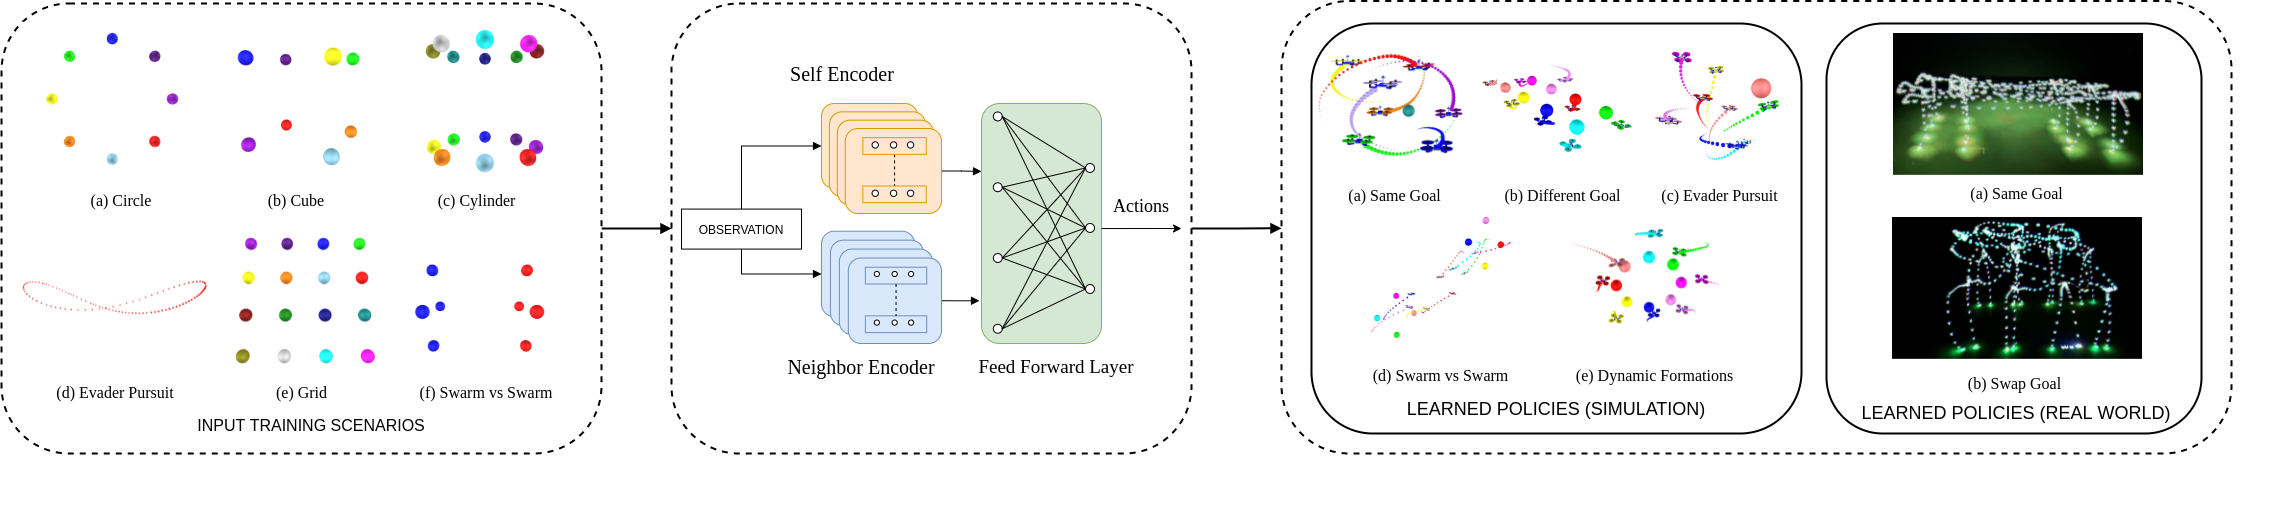
\includegraphics[width=0.7\textwidth]{literature/batra2021_fig1}
  \caption[Decentralised quadrotor-swarm control with shared encoders (Batra et al.)]{Decentralised
  quadrotor-swarm control with self and neighbour encoders trained on randomised formation scenarios.
  Reproduced from Batra et al.\ \cite{batra2021decentralized}.}
  \label{fig:lit_batra}
\end{figure}

Huang et al.\ \cite{huang2024collision} extended this line of work to navigation through obstacle fields. They
add an obstacle encoder, use attention over neighbour and obstacle observations, and introduce a replay mechanism
that restarts training episodes from states shortly before a collision, so that the policy practises difficult
situations more often while still collecting fresh on-policy data. The accompanying QuadSwarm simulator
\cite{huang2023quadswarm} emphasises the separation of the simulation from rendering and a seeded, randomised
generation of scenarios. Our observation structure (self, neighbours, objects), the attention encoders, the
collision-state replay and the separation of the simulator from the web viewer follow these works.

\section{Simulation Environments for Multi-Drone Learning}
Panerati et al.\ \cite{panerati2021learning} introduced gym-pybullet-drones, a multi-agent quadcopter environment
with rigid-body physics and aerodynamic effects, and discussed the choice of the control level at which an RL
agent acts, from motor commands to velocity set-points. This motivates the decision in this project to learn at
the velocity level above a stabilised flight model, which makes training fast enough for ordinary hardware, and
identifies a path for later validation with full quadrotor physics.

\section{Collision Avoidance and Learning from Demonstrations}
Van den Berg et al.\ \cite{vandenberg2011reciprocal} formulated reciprocal collision avoidance for many agents in
terms of the relative positions and velocities of neighbouring agents. Reasoning about relative motion over a
short prediction horizon underlies both the observation design of our policy and the sampling-based expert
planner that provides demonstrations.

Learning from demonstrations reduces the exploration that RL must perform. Plain behaviour cloning suffers from
covariate shift: the learner makes small errors, reaches states that the expert never demonstrated and does not
know how to recover. DAgger \cite{ross2011reduction} removes this problem by letting the learner act, asking the
expert to label every state the learner visits, and training on the aggregated data set. Our pipeline uses DAgger
rounds at the start of every curriculum stage.

\section{Research Gap}
The reviewed swarm-RL works \cite{batra2021decentralized,huang2024collision} learn directly at the thrust level
with very large sample budgets, and their formation tasks do not require a drone to return to its own slot after
an avoidance manoeuvre. Three aspects motivate the present project:
\begin{enumerate}
  \item \textbf{Same-slot recovery as an explicit requirement.} After avoiding an object, each drone must return
        to its own slot relative to a moving target, measured with a quantitative recovery criterion.
  \item \textbf{Training on ordinary hardware.} By learning coordination above a stabilised flight layer
        \cite{panerati2021learning} and initialising each curriculum stage from expert demonstrations
        \cite{ross2011reduction}, the complete training runs on a laptop in a few hours.
  \item \textbf{Held-out, reproducible evaluation.} Training, checkpoint selection and final testing use disjoint
        ranges of random seeds, and every reported number is regenerated from saved files.
\end{enumerate}
